\documentclass[9pt,twocolumn,twoside]{styles/osajnl}
\usepackage{fancyvrb}
\journal{i524} 

\title{Nagios - Example Paper for I524}

\author[1]{Tony Liu}
\author[1]{Vibhatha Abeykoon}
\author[1]{Gregor von Laszewski}

\affil[1]{School of Informatics and Computing, Bloomington, IN 47408, U.S.A.}


\dates{paper-1, \today}

\ociscodes{Cloud, I524}

% replace this with your url in github/gitlab
\doi{\url{https://github.com/vibhatha/sp17-i524/blob/master/paper1/S17-TS-0003/report.pdf}}


\begin{abstract}
This paper is an example research article for I524, written under the example template. 
We selected Techlist 363, Nagios, as the topic to demonstrate how to properly compose a research
article.
Nagios is a platform/tool, which provides a set of software for system and network infrastructure monitoring. Within this article, we explored what problem it tried to solve, how it solved the problem, and why it's important to have Nagios. We also discussed the advantages and disadvantages it possessed. 
\end{abstract}

\setboolean{displaycopyright}{true}

\begin{document}

\maketitle

\section{Introduction}

According to ~\cite{nagios-book}, even through the machines have become more and 
more critical to us human being, they are untrustworthy. I just couldn't agree more with the author. Look at the GitLab.com incident happened on Jan 31st 2017. A tired system administrator, working late at night in the Netherlands, had accidentally deleted a directory on the wrong server during a frustrating database replication process: he wiped a folder containing 300GB of live production data that was due to be replicated~\cite{gitlabmeltdown}. Mistakes could be corrected easily since Gitlab have deployed several methods to backup and replicate the production data and all they just need to  do is to recover and restore from the backup. However, after several attempts, they found that out of 5 backup/replication techniques deployed none were working reliably or set up in the first place.


\section{What is Nagios}

Nagios is a system and network monitoring tool under open source license that provides instant awareness of mission-critical IT infrastructure. Nagios allows to monitor the infrastructure, alert the system admin, provide visualized reports, schedule downtime for maintenance, and plan upgrade in advance with trends and capacity diagrams. Its design emphasizes highly on flexibility and scalability. To provide such flexibility, Nagios is composed of different modules. The reason behind this modular design is that Nagios fully considers the variety of systems and networks it will monitor on. Different customers require a large amount of customization before they themselves know they do.



\section{Why is Nagios Important}

This section discusses why is Nagios important and why we need it.
Elaborate Nagios' features with Gitlab example in the introduction.
Modular. Scalable. Adaptable.

\label{sec:examples}

The sections below show examples of different article components.

\section{Advantages and Disadvantages}

We will dig more on Nagios by take a look at its architecture.

\subsection{Sample Figure}

Figure \ref{fig:nagios-architecture} shows an example figure.

\begin{figure}[htbp]
\centering
\fbox{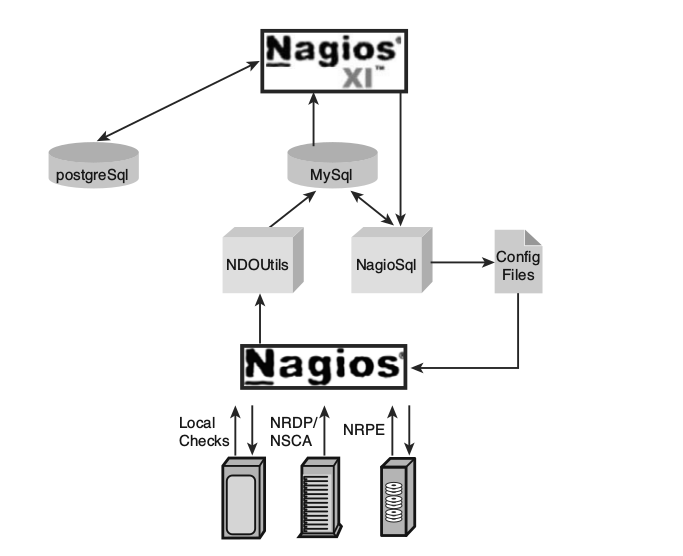
\includegraphics[width=\linewidth]{images/nagios-architecture}}
\caption{Nagios Architecture}
\label{fig:nagios-architecture}
\end{figure}



\section{Conclusion}


With the Gitlab incidence, we can see how untrustworthy the machines can be. This is also why we need Nagios.



% Bibliography

\bibliography{references}
 
%\newpage

\appendix


\section{Work Breakdown}

The work on this project was distributed as follows between the
authors:

\begin{description}

\item[John Smith.] Explored the deep mathematical knowledge needed for
  this paper and taught it to the other authors.

\item[Alice Smith.] She explored the world of Oz and was instrumental
  to work on the deployment of hadoop.

\item[Bruce Wayne.] He did not contribute at all to this paper and
  flew around to safe the world.  

\end{description}

\section{Report Checklist}

\begin{itemize}
\renewcommand{\labelitemi}{\scriptsize$\square$} 
\item Have you written the report in word or LaTeX in the specified
  format?
\item Have you included the report in github/lab?
\item Have you specified the names and e-mails of all team members in
  your report. E.g. the username in Canvas?
\item Have you included the HID of all team members?
\item Does the report have the project number added to it?
\item Have you included all images in native and PDF format in gitlab
  in the images folder?
\item Have you added the bibliography file in bibtex format?
\item Have you submitted an additional page that describes who did
  what in the project or report?
\item Have you spellchecked the paper?
\item Have you made sure you do not plagiarize?
\item Have you made sure that the important directories are all lower
  case and have no underscore or space in it?
\item Have you made sure that all authors have a README.rst in their
  HID github/lab repository?
\item Have you made sure that there is a README.rst in the project
  directory and that it is properly filled out?
\item Have you put a work breakdown in the document if you worked in a
  group?
\end{itemize}

\section{Possible technology paper outline}

The next sections are just some suggestions, your may want to add
sections and subsections as you see fit. Images and references do not
count towards the 2 page length. Please use the \verb|\section|,
\verb|\subsection|, and \verb|\subsubsection| commands in your
paper. do not introduce hardcoded numbers. Use the \verb|\ref| and
\verb|\label| commands to refer
 to the sections.


\paragraph{Abstract}

Put in the abstract a summary what this paper is about

\paragraph{1. Introduction}

Introduce the technology and provide general useful information.

\paragraph{2. Architecture} 

If applicable include a description about architectural details. This
may include a figure. Make sure that if you copy a figure you put the
\cite{?} in the caption also. Otherwise it is plagiarism.

\paragraph{2.1. API}

comment on the API which could include language bindings

\paragraph{2.2. Shell Access}

If applicable comment on how the tool can be used from the command line

\paragraph{2.3.Graphical Interface}

If applicable comment on if the technology has a GUI

\paragraph{3. Licensing}

Often tools may have different versions, some fre, some for
pay. Comment on this. For example while a tool may offer a comercial
version this version may be too costly for others. Identify especially
the difference between features for free vs commercial tools.

Sometimes you may need to introduce this also in the introduction as
there may be a big difference and without the knowledge you do not
provide the user an adequate introduction.

\paragraph{4. Ecosystem}

Some technologies have a large ecosystem developed around them with
extensions plugins and other useful tools. Identify if they exists and
comment on what they can achieve

provide potentially a mindmap or a figure illustrating how the
technology fits in with other technologies if applicable.

\paragraph{4. Use Cases}

\paragraph{4.1. Use Cases  for Big Data}

Locate and describe major usecases that demonstrate the technology
while focussing on big data related use cases. Make sure you do proper
references with the \cite{?} command. Do not put URLs in the text.

\paragraph {4.2. Other Use Cases}

Some technologies may not just be used for big data, find other makor
use cases from other areas if applicable.  Make sure you do proper
references with the \cite{?} command. Do not put URLs in the text.

\paragraph{5. Educational material}

Put information here how someone would find out more about the
technology. Use important material and do not list hundrets of web
pages, be selective.

\paragraph{6. Conclusion}

Put in some conclusion based on what you have researched

\paragraph{Acknowledgement}

Put in the information for this class and who may sponsor
you. Examples will be given later

\end{document}
